\documentclass[12pt]{article}

\usepackage{sbc-template}
\usepackage{graphicx,url}
\usepackage{multirow}
\usepackage[table,xcdraw]{xcolor}
\usepackage{lscape}
\usepackage{longtable}
\usepackage{pgfplots}
\pgfplotsset{width=10cm,compat=1.9}
\usepgfplotslibrary{external}
\tikzexternalize
\usepackage[utf8]{inputenc}
\usepackage[brazil]{babel}
\usepackage[latin1]{inputenc}  

\usepackage{listings}
\usepackage{color}

%New colors defined below
\definecolor{codegreen}{rgb}{0,0.6,0}
\definecolor{codegray}{rgb}{0.5,0.5,0.5}
\definecolor{codepurple}{rgb}{0.58,0,0.82}
\definecolor{backcolour}{rgb}{0.95,0.95,0.92}

%Code listing style named "mystyle"
\lstdefinestyle{mystyle}{
  backgroundcolor=\color{backcolour},   commentstyle=\color{codegreen},
  keywordstyle=\color{blue},
  numberstyle=\tiny\color{codegray},
  stringstyle=\color{codepurple},
  basicstyle=\footnotesize,
  breakatwhitespace=false,         
  breaklines=true,                 
  captionpos=b,                    
  keepspaces=true,                 
  numbers=left,                    
  numbersep=5pt,                  
  showspaces=false,                
  showstringspaces=false,
  showtabs=false,                  
  tabsize=2
}
\lstset{style=mystyle}
\sloppy

\title{Comparison between algorithms for the shortest pathproblem\\ }
\author{Karelia A. Vilca\inst{1}}

\address{Instituto de Ciências Matemáticas e de Computação -- Universidade de São Paulo
  (USP) \\ -- São Carlos, SP -- Brazil\\
  \email{\ karelia@usp.br}
}

\begin{document} 

\maketitle

\begin{abstract}
  This meta-paper describes the style to be used in articles and short papers
  for SBC conferences. For papers in English, you should add just an abstract
  while for the papers in Portuguese, we also ask for an abstract in
  Portuguese (``resumo''). In both cases, abstracts should not have more than
  10 lines and must be in the first page of the paper.
\end{abstract}
     
\begin{resumo} 
  Este meta-artigo descreve o estilo a ser usado na confecção de artigos e
  resumos de artigos para publicação nos anais das conferências organizadas
  pela SBC. É solicitada a escrita de resumo e abstract apenas para os artigos
  escritos em português. Artigos em inglês deverão apresentar apenas abstract.
  Nos dois casos, o autor deve tomar cuidado para que o resumo (e o abstract)
  não ultrapassem 10 linhas cada, sendo que ambos devem estar na primeira
  página do artigo.
\end{resumo}


\section{General Information}

All full papers and posters (short papers) submitted to some SBC conference,
including any supporting documents, should be written in English or in
Portuguese. The format paper should be A4 with single column, 3.5 cm for upper
margin, 2.5 cm for bottom margin and 3.0 cm for lateral margins, without
headers or footers. The main font must be Times, 12 point nominal size, with 6
points of space before each paragraph. Page numbers must be suppressed.

Full papers must respect the page limits defined by the conference.
Conferences that publish just abstracts ask for \textbf{one}-page texts.


\section{Algoritmos}

\subsection{DFS}
\cite{tarjan1972depth}
\lstinputlisting[language=C++, caption=DFS algorithm]{codes/DFS.hpp}
%\clearpage
\subsection{BFS}
\lstinputlisting[language=C++, caption=BFS algorithm]{codes/BFS.hpp}

\subsection{A*}
\lstinputlisting[language=C++, caption=A* algorithm]{codes/Aasterisk.hpp}

\subsection{Hill Climbing}
\lstinputlisting[language=C++, caption=Hill Climbing algorithm]{codes/HillClimbing.hpp}

\subsection{Comparision}
\begin{lstlisting}[language=C++, caption=Build graph and tree]
void Build_graph()
{	
	//Empty matrix
	vector<float> vect;	
	for(int i=0; i<dots.size();i++)
		vect.push_back(0);	
	for(int i=0; i<dots.size();i++)
		grafo.push_back(vect);
	float d;
	//Adjacence matrix
	for(int i=0; i<dots.size();i++)
	{	vector<int> adj;
		for(int j=0; j<dots.size();j++)
		{   
			d=distance(dots[i].first,dots[j].first,dots[i].second,dots[j].second);
			if(d<limit)
			{
				grafo[i][j]=d;
				edges.push_back(make_pair(make_pair(dots[i].first,dots[i].second),make_pair(dots[j].first,dots[j].second)));///Grafico
				adj.push_back(j);
			}
		}
		graph.push_back(adj);
	}
}

void Build_tree()
{
	for(int i=0; i<dots.size();i++)
	{	
		vector<int> sons;
		for(int j=i; j<dots.size();j++)
		{
			if(grafo[i][j]<limit)
				sons.push_back(j);
		}
		tree.push_back(sons);
	}	
}
\end{lstlisting}
\begin{lstlisting}[language=C++, caption=Build graph and tree]
    cout<<"Number of dots"<<endl;
    cin>>N_DOTS;
    cout<<endl<<"Complete graph? (y/n)"<<endl;
    char yn;
    cin>>yn;
    if(yn=='n')limit=N_DOTS*0.8;
    cout<<endl<<"Press key to algorithm path"<<endl;
    cout<<"d ---> DFS "<<endl; 
    cout<<"b ---> BFS "<<endl;
    cout<<"a ---> A* "<<endl;
    cout<<"h ---> Hill Climbing "<<endl;
    
    srand(time(NULL));
    ///Random dots
    for(int i=0; i<N_DOTS; ++i)
    {
        float auxx=rand()%N_DOTS-rand()%N_DOTS;
        float auxy=rand()%N_DOTS-rand()%N_DOTS;
		dots.push_back(make_pair(auxx,auxy));
    }
    coord_ini=0;
    coord_fin=rand()%N_DOTS;
    start = dots[coord_ini];
    meta = dots[coord_fin];
    
    Build_graph();
    Build_tree();
  	Algorithms();
\end{lstlisting}
\section{First Page} \label{sec:firstpage}

The first page must display the paper title, the name and address of the
authors, the abstract in English and ``resumo'' in Portuguese (``resumos'' are
required only for papers written in Portuguese). The title must be centered
over the whole page, in 16 point boldface font and with 12 points of space
before itself. Author names must be centered in 12 point font, bold, all of
them disposed in the same line, separated by commas and with 12 points of
space after the title. Addresses must be centered in 12 point font, also with
12 points of space after the authors' names. E-mail addresses should be
written using font Courier New, 10 point nominal size, with 6 points of space
before and 6 points of space after.

The abstract and ``resumo'' (if is the case) must be in 12 point Times font,
indented 0.8cm on both sides. The word \textbf{Abstract} and \textbf{Resumo},
should be written in boldface and must precede the text.

\section{CD-ROMs and Printed Proceedings}

In some conferences, the papers are published on CD-ROM while only the
abstract is published in the printed Proceedings. In this case, authors are
invited to prepare two final versions of the paper. One, complete, to be
published on the CD and the other, containing only the first page, with
abstract and ``resumo'' (for papers in Portuguese).

\section{Sections and Paragraphs}

Section titles must be in boldface, 13pt, flush left. There should be an extra
12 pt of space before each title. Section numbering is optional. The first
paragraph of each section should not be indented, while the first lines of
subsequent paragraphs should be indented by 1.27 cm.

\subsection{Subsections}

The subsection titles must be in boldface, 12pt, flush left.

\section{Figures and Captions}\label{sec:figs}


Figure and table captions should be centered if less than one line
(Figure~\ref{fig:exampleFig1}), otherwise justified and indented by 0.8cm on
both margins, as shown in Figure~\ref{fig:exampleFig2}. The caption font must
be Helvetica, 10 point, boldface, with 6 points of space before and after each
caption.

\begin{figure}[ht]
\centering
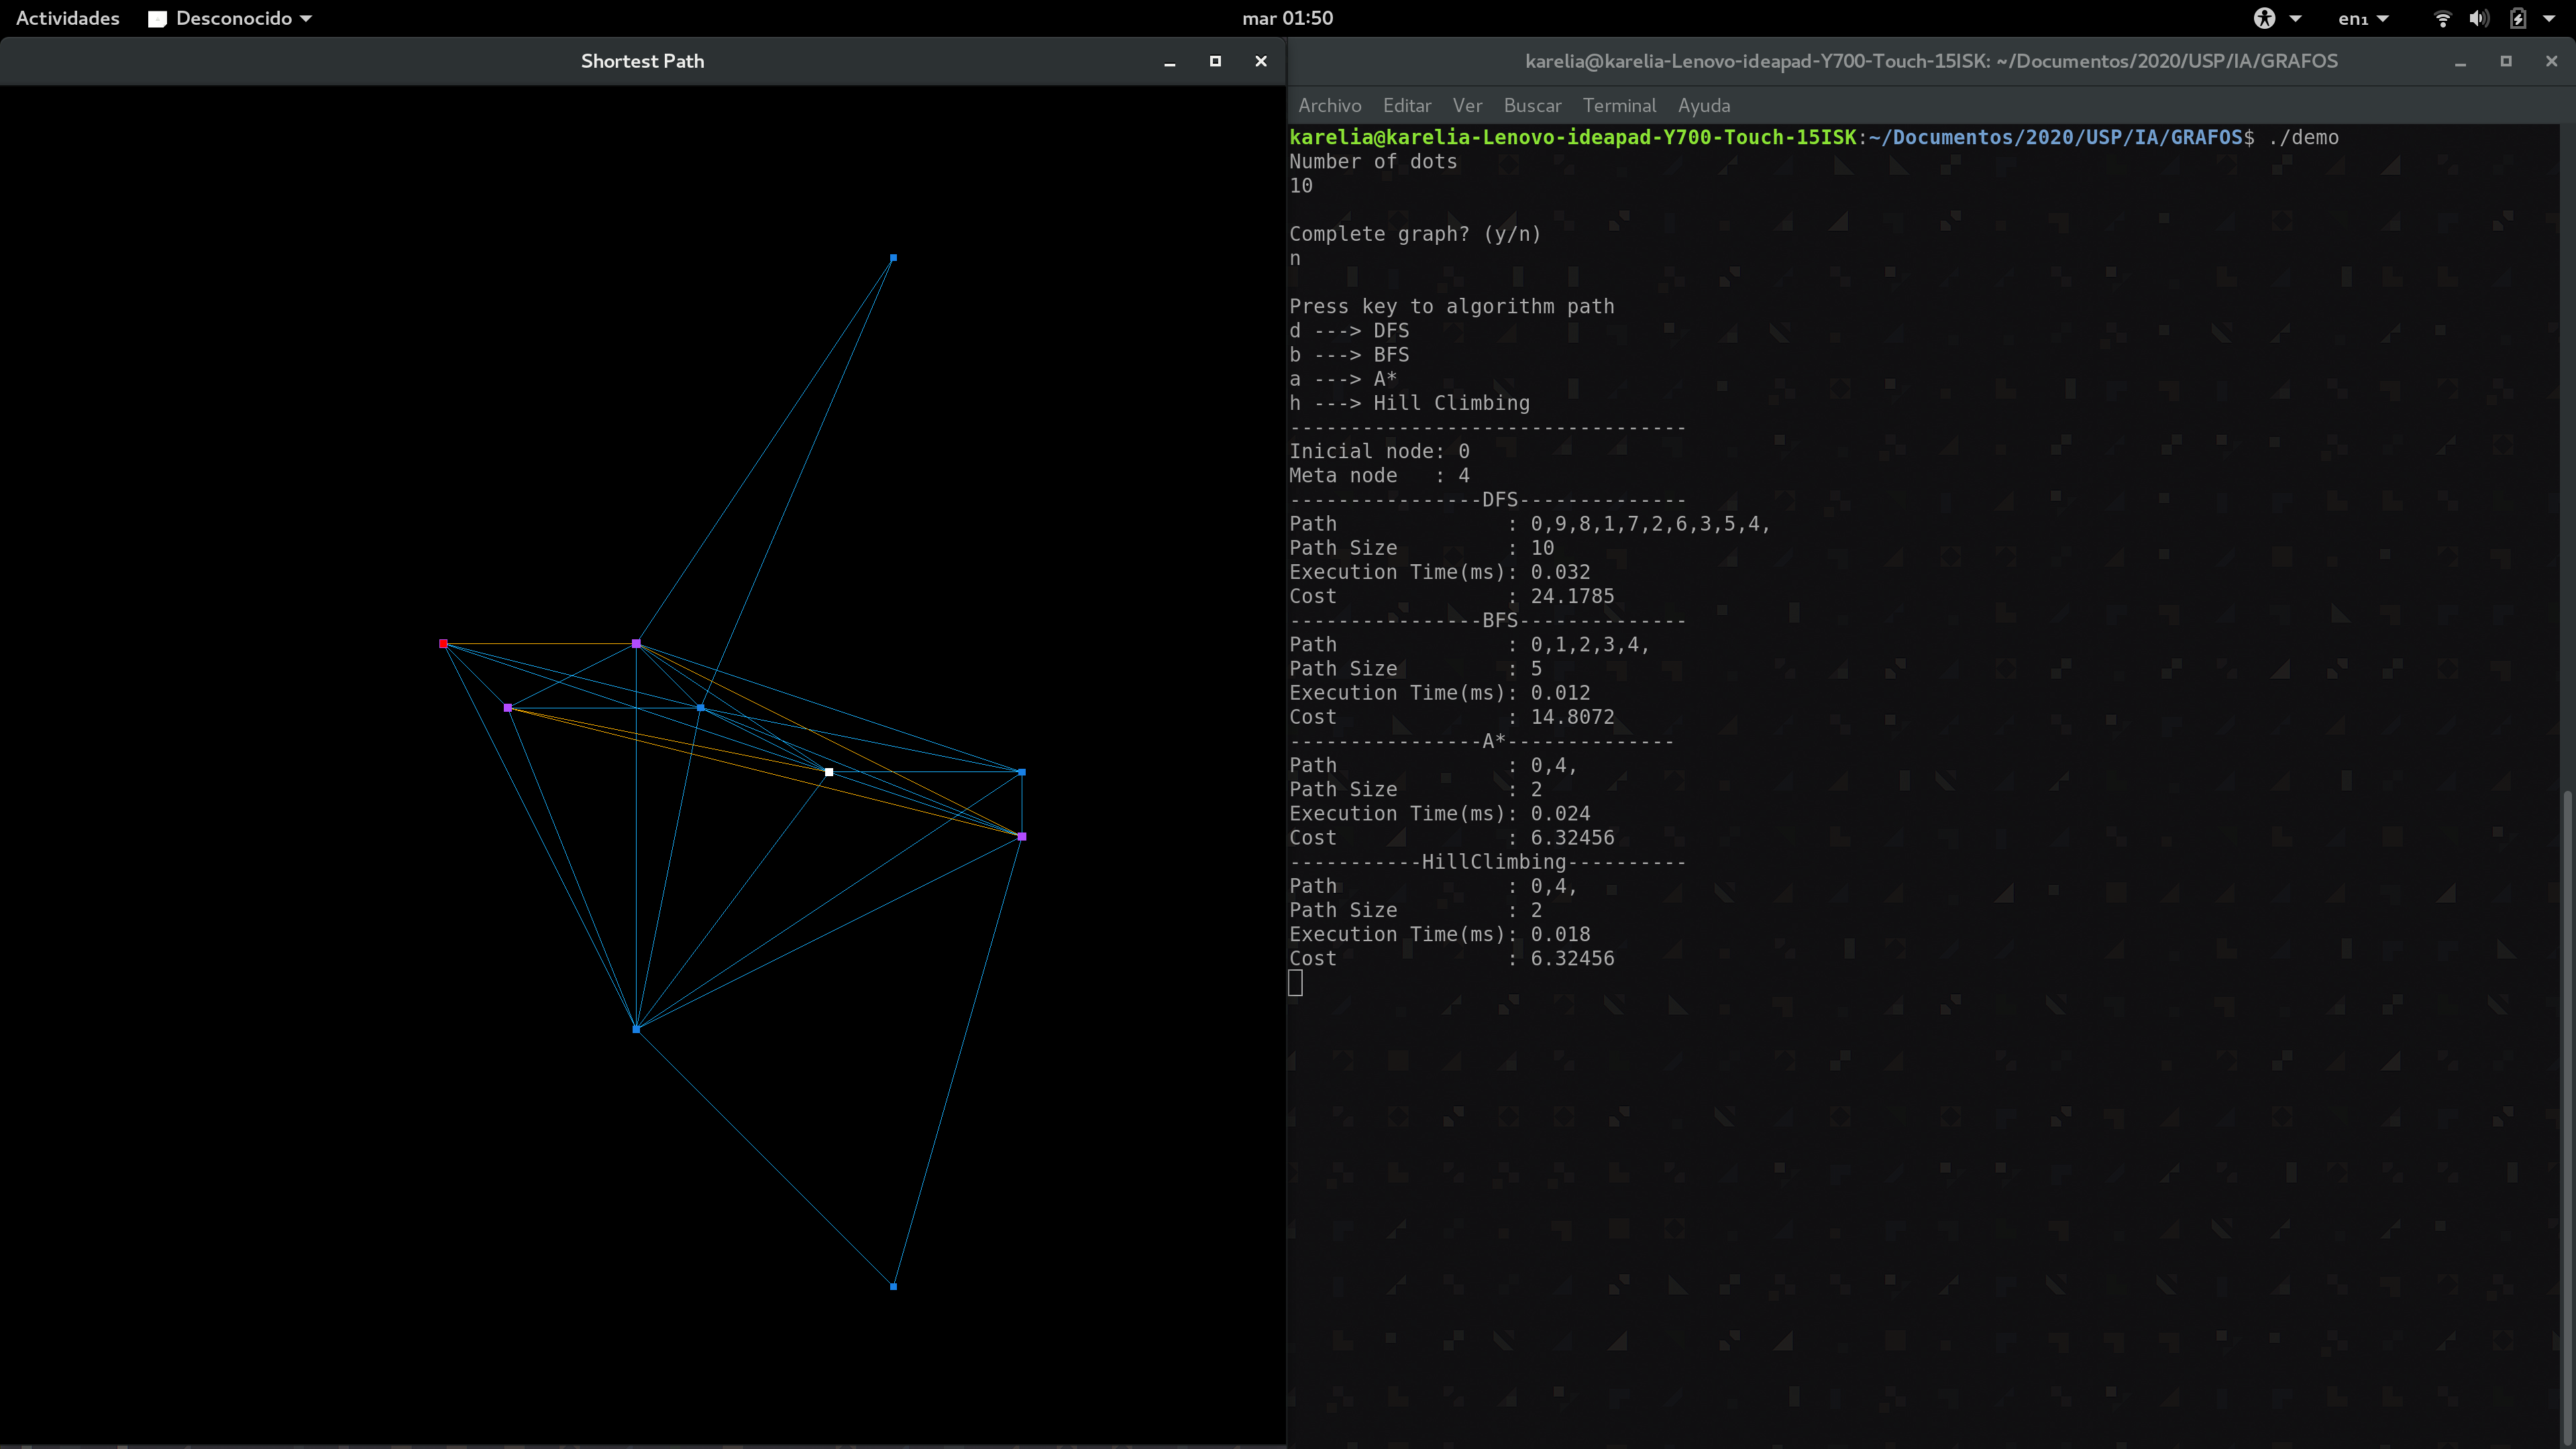
\includegraphics[width=1.0\textwidth]{Template_SBC/template-latex/screen1.png}
\caption{A typical figure}
\label{fig:exampleFig1}
\end{figure}

\begin{figure}[ht]
\centering
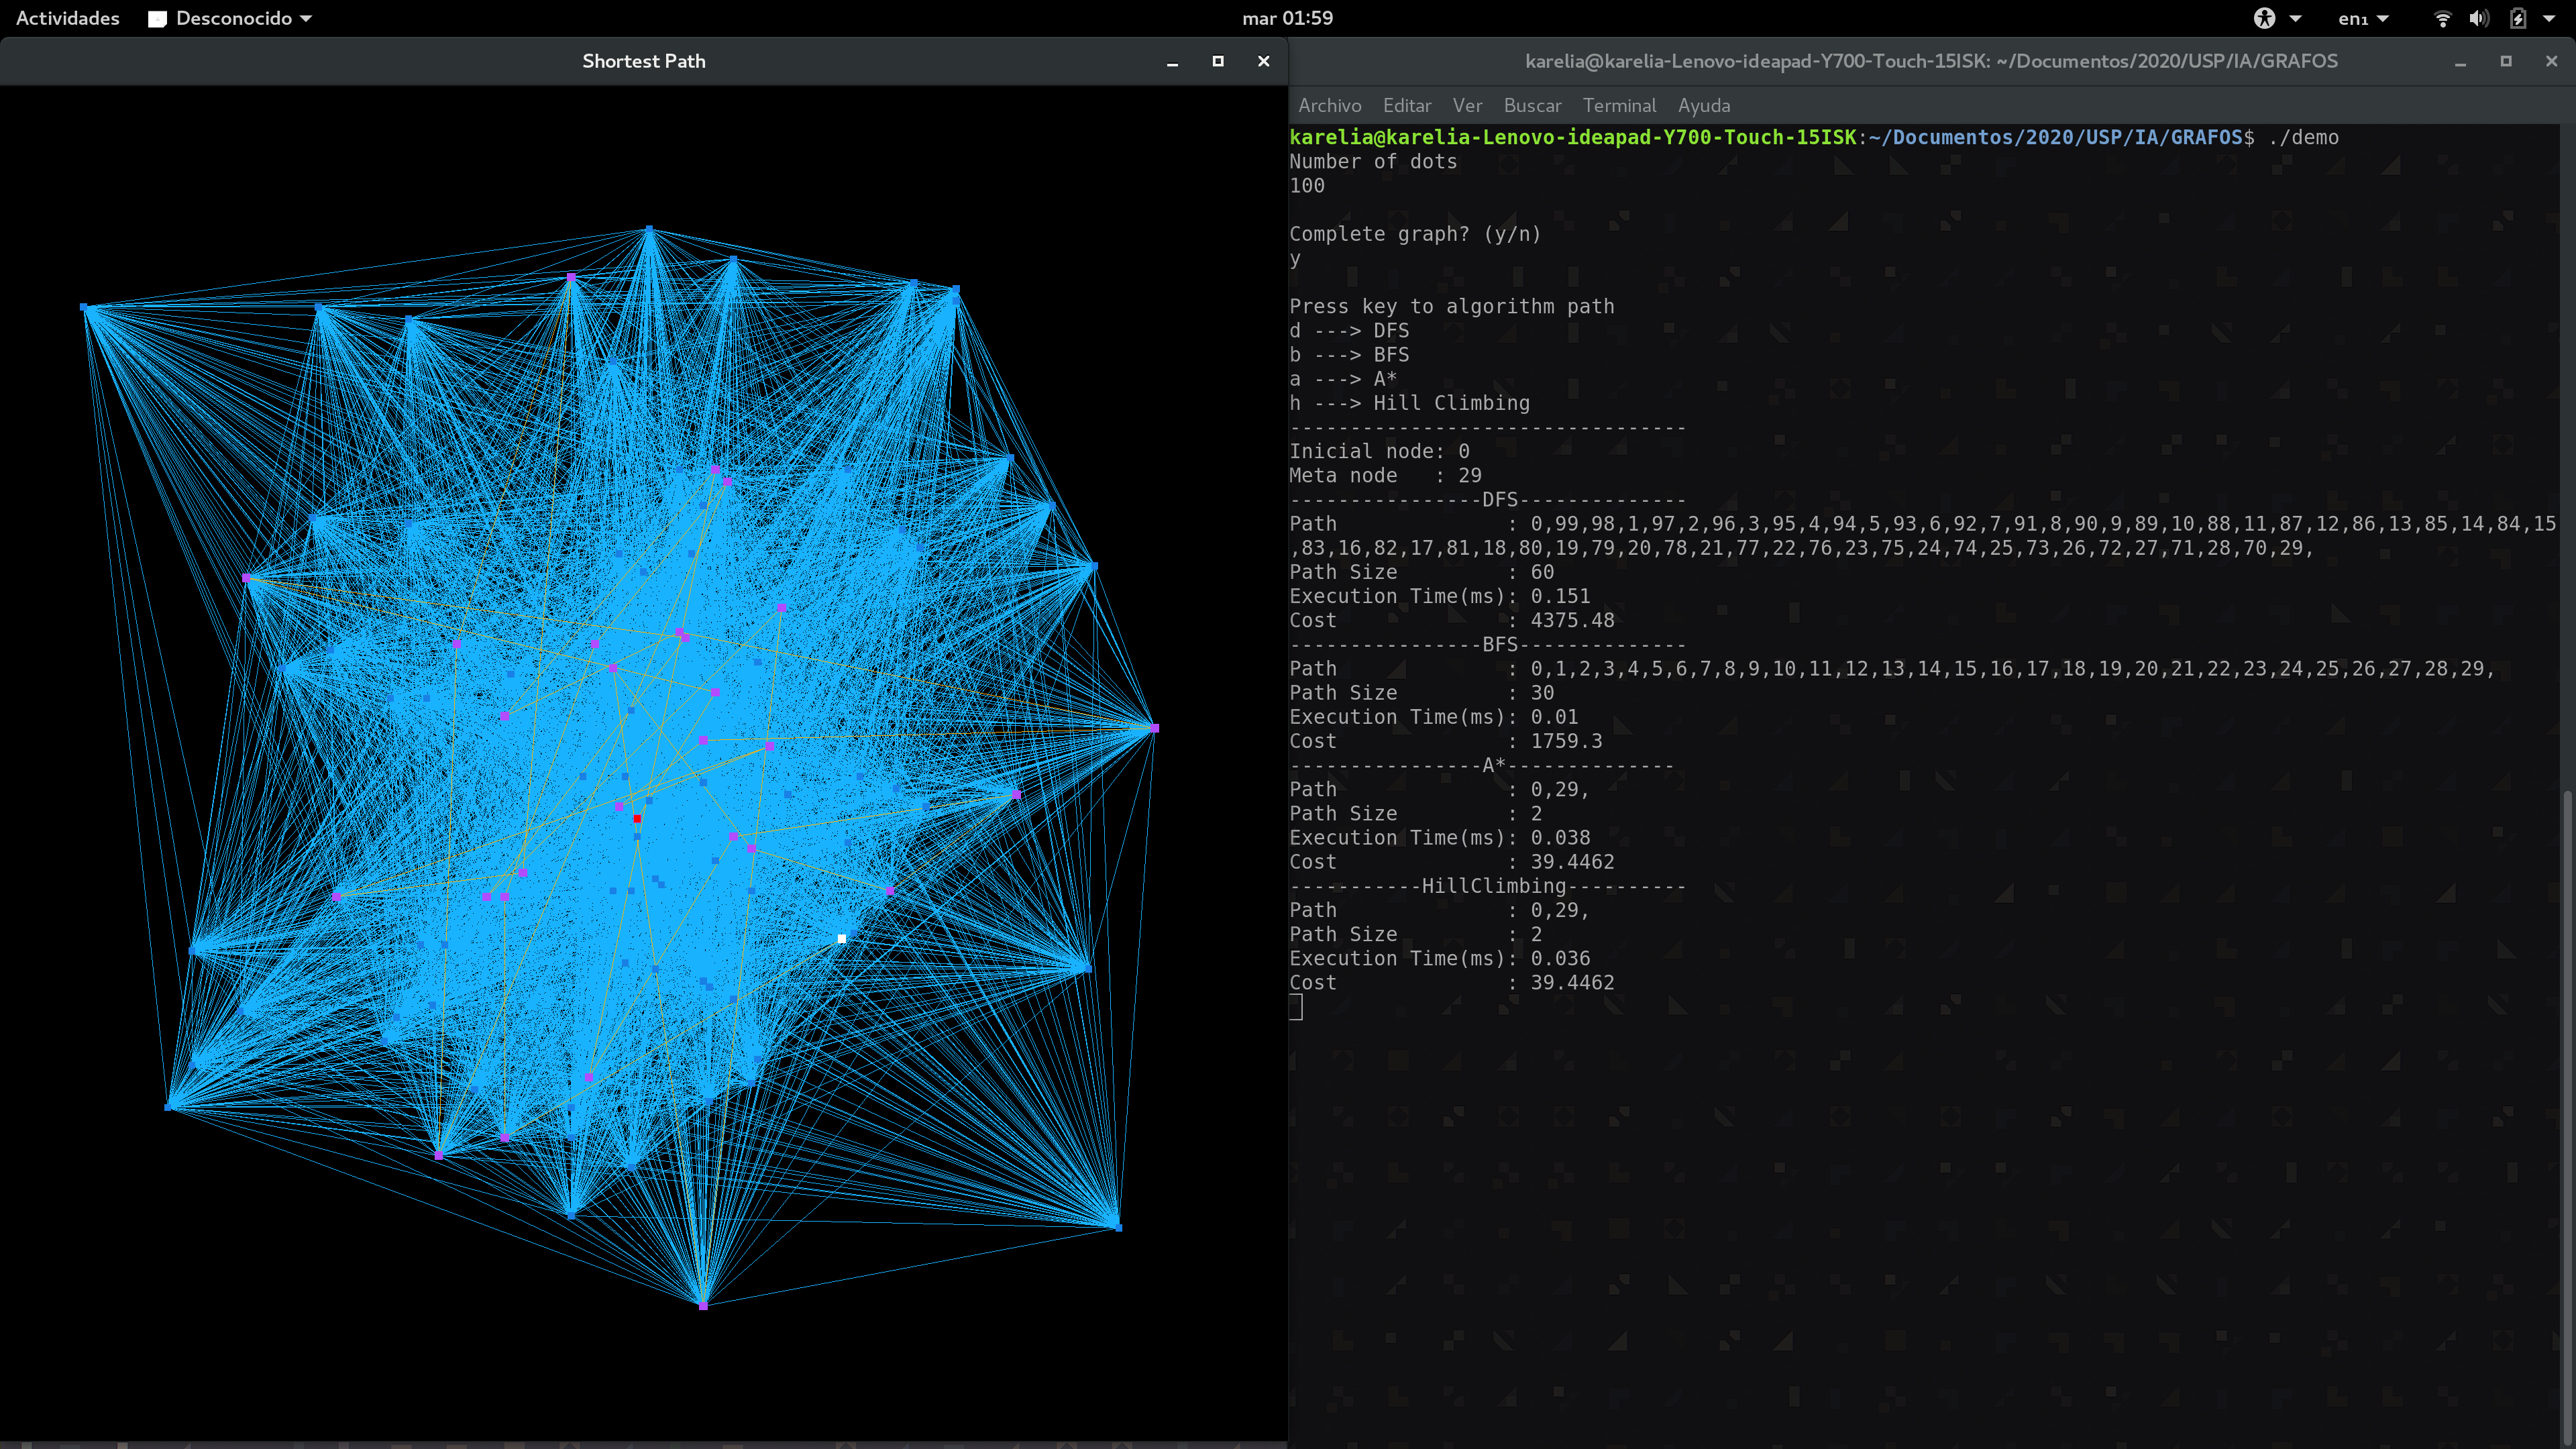
\includegraphics[width=1.0\textwidth]{Template_SBC/template-latex/screen2.png}
\caption{This figure is an example of a figure caption taking more than one
  line and justified considering margins mentioned in Section~\ref{sec:figs}.}
\label{fig:exampleFig2}
\end{figure}

In tables, try to avoid the use of colored or shaded backgrounds, and avoid
thick, doubled, or unnecessary framing lines. When reporting empirical data,
do not use more decimal digits than warranted by their precision and
reproducibility. Table caption must be placed before the table (see Table 1)
and the font used must also be Helvetica, 10 point, boldface, with 6 points of
space before and after each caption.

\begin{table}[ht]
\centering
\caption{Variables to be considered on the evaluation of interaction
  techniques}
\label{tab:exTable1}
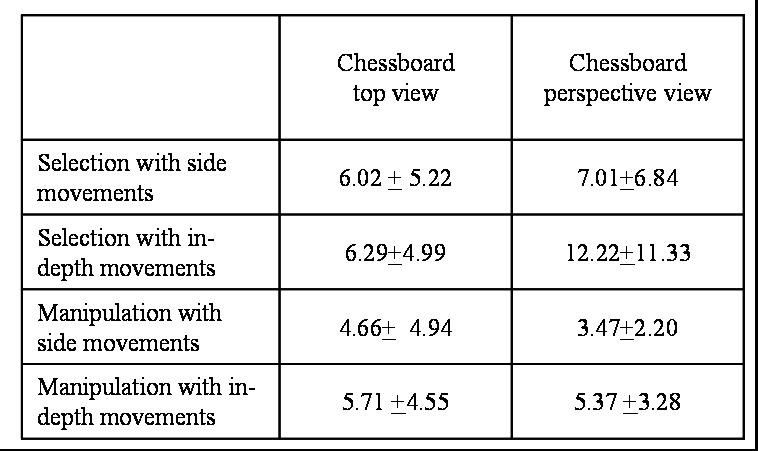
\includegraphics[width=.7\textwidth]{table.jpg}
\end{table}

\section{Images}

All images and illustrations should be in black-and-white, or gray tones,
excepting for the papers that will be electronically available (on CD-ROMs,
internet, etc.). The image resolution on paper should be about 600 dpi for
black-and-white images, and 150-300 dpi for grayscale images.  Do not include
images with excessive resolution, as they may take hours to print, without any
visible difference in the result. 
\section{Results}
% Please add the following required packages to your document preamble:
% \usepackage{multirow}
% \usepackage[table,xcdraw]{xcolor}
% If you use beamer only pass "xcolor=table" option, i.e. \documentclass[xcolor=table]{beamer}
% \usepackage{lscape}
% \usepackage{longtable}
% Note: It may be necessary to compile the document several times to get a multi-page table to line up properly
\begin{landscape}
\begin{longtable}[c]{|c|c|l|l|l|l|l|l|l|l|l|l|l|l|}
\hline
\multicolumn{2}{|c|}{} &
  \multicolumn{6}{c|}{\textbf{Blind}} &
  \multicolumn{6}{c|}{\textbf{Heuristic}} \\ \cline{3-14} 
\multicolumn{2}{|c|}{\multirow{-2}{*}{\textbf{Search}}} &
  \multicolumn{3}{c|}{\textbf{DFS}} &
  \multicolumn{3}{c|}{\textbf{BFS}} &
  \multicolumn{3}{c|}{\textbf{A*}} &
  \multicolumn{3}{c|}{\textbf{Hill Climbing}} \\ \hline
\endhead
%
\multicolumn{2}{|c|}{\textbf{Features}} &
  \multicolumn{1}{c|}{} &
  \multicolumn{1}{c|}{} &
  \multicolumn{1}{c|}{} &
  \multicolumn{1}{c|}{} &
  \multicolumn{1}{c|}{} &
  \multicolumn{1}{c|}{} &
  \multicolumn{1}{c|}{} &
  \multicolumn{1}{c|}{} &
  \multicolumn{1}{c|}{} &
  \multicolumn{1}{c|}{} &
  \multicolumn{1}{c|}{} &
  \multicolumn{1}{c|}{} \\ \cline{1-2}
\textbf{\#N} &
  \textbf{Comp.} &
  \multicolumn{1}{c|}{\multirow{-2}{*}{\textbf{\begin{tabular}[c]{@{}c@{}}Path\\ size\end{tabular}}}} &
  \multicolumn{1}{c|}{\multirow{-2}{*}{\textbf{\begin{tabular}[c]{@{}c@{}}E.Time\\ (ms)\end{tabular}}}} &
  \multicolumn{1}{c|}{\multirow{-2}{*}{\textbf{Cost}}} &
  \multicolumn{1}{c|}{\multirow{-2}{*}{\textbf{\begin{tabular}[c]{@{}c@{}}Path\\ size\end{tabular}}}} &
  \multicolumn{1}{c|}{\multirow{-2}{*}{\textbf{\begin{tabular}[c]{@{}c@{}}E.Time\\ (ms)\end{tabular}}}} &
  \multicolumn{1}{c|}{\multirow{-2}{*}{\textbf{Cost}}} &
  \multicolumn{1}{c|}{\multirow{-2}{*}{\textbf{\begin{tabular}[c]{@{}c@{}}Path\\ size\end{tabular}}}} &
  \multicolumn{1}{c|}{\multirow{-2}{*}{\textbf{\begin{tabular}[c]{@{}c@{}}E.Time\\ (ms)\end{tabular}}}} &
  \multicolumn{1}{c|}{\multirow{-2}{*}{\textbf{Cost}}} &
  \multicolumn{1}{c|}{\multirow{-2}{*}{\textbf{\begin{tabular}[c]{@{}c@{}}Path\\ size\end{tabular}}}} &
  \multicolumn{1}{c|}{\multirow{-2}{*}{\textbf{\begin{tabular}[c]{@{}c@{}}E.Time\\ (ms)\end{tabular}}}} &
  \multicolumn{1}{c|}{\multirow{-2}{*}{\textbf{Cost}}} \\ \hline
 &
  \textbf{Y} &
  3 &
  0.022 &
  15.1333 &
  9 &
  0.02 &
  67.2523 &
  \cellcolor[HTML]{C0C0C0}2 &
  0.023 &
  \cellcolor[HTML]{C0C0C0}2.23607 &
  \cellcolor[HTML]{C0C0C0}{\color[HTML]{00009B} 2} &
  \cellcolor[HTML]{C0C0C0}{\color[HTML]{00009B} 0.19} &
  \cellcolor[HTML]{C0C0C0}{\color[HTML]{00009B} 2.23607} \\ \cline{2-14} 
\multirow{-2}{*}{\textbf{10}} &
  \textbf{N} &
  10 &
  0.032 &
  24.1785 &
  5 &
  \cellcolor[HTML]{C0C0C0}0.012 &
  14.8072 &
  \cellcolor[HTML]{C0C0C0}2 &
  0.024 &
  \cellcolor[HTML]{C0C0C0}6.32456 &
  \cellcolor[HTML]{C0C0C0}{\color[HTML]{00009B} 2} &
  \cellcolor[HTML]{FFFFFF}{\color[HTML]{00009B} 0.018} &
  \cellcolor[HTML]{C0C0C0}{\color[HTML]{00009B} 6.32456} \\ \hline
 &
  \textbf{Y} &
  7 &
  \cellcolor[HTML]{C0C0C0}0.055 &
  254.153 &
  47 &
  0.061 &
  1645.44 &
  \cellcolor[HTML]{C0C0C0}2 &
  0.086 &
  \cellcolor[HTML]{C0C0C0}44.6878 &
  \cellcolor[HTML]{C0C0C0}{\color[HTML]{00009B} 2} &
  {\color[HTML]{00009B} 0.08} &
  \cellcolor[HTML]{C0C0C0}{\color[HTML]{00009B} 44.6878} \\ \cline{2-14} 
\multirow{-2}{*}{\textbf{50}} &
  \textbf{N} &
  13 &
  0.067 &
  166.22 &
  44 &
  \cellcolor[HTML]{C0C0C0}0.045 &
  715.09 &
  \cellcolor[HTML]{C0C0C0}3 &
  0.07 &
  \cellcolor[HTML]{C0C0C0}19.9561 &
  \cellcolor[HTML]{C0C0C0}{\color[HTML]{00009B} 3} &
  {\color[HTML]{00009B} 0.063} &
  \cellcolor[HTML]{C0C0C0}{\color[HTML]{00009B} 19.9561} \\ \hline
 &
  \textbf{Y} &
  60 &
  0.151 &
  4375.48 &
  30 &
  \cellcolor[HTML]{C0C0C0}0.01 &
  1759.3 &
  \cellcolor[HTML]{C0C0C0}2 &
  0.038 &
  \cellcolor[HTML]{C0C0C0}39.4462 &
  \cellcolor[HTML]{C0C0C0}{\color[HTML]{00009B} 2} &
  {\color[HTML]{00009B} 0.033} &
  \cellcolor[HTML]{C0C0C0}{\color[HTML]{00009B} 39.4462} \\ \cline{2-14} 
\multirow{-2}{*}{\textbf{100}} &
  \textbf{N} &
  46 &
  0.104 &
  1439.16 &
  23 &
  \cellcolor[HTML]{C0C0C0}0.008 &
  650.663 &
  {\color[HTML]{036400} 4} &
  {\color[HTML]{036400} 0.039} &
  \cellcolor[HTML]{C0C0C0}{\color[HTML]{036400} 101.829} &
  \cellcolor[HTML]{C0C0C0}3 &
  0.034 &
  109.776 \\ \hline
 &
  \textbf{Y} &
  42 &
  0.454 &
  14382.9 &
  21 &
  \cellcolor[HTML]{C0C0C0}0.007 &
  8103.29 &
  \cellcolor[HTML]{C0C0C0}2 &
  0.592 &
  \cellcolor[HTML]{C0C0C0}432.334 &
  \cellcolor[HTML]{C0C0C0}{\color[HTML]{00009B} 2} &
  {\color[HTML]{00009B} 0.192} &
  \cellcolor[HTML]{C0C0C0}{\color[HTML]{00009B} 432.334} \\ \cline{2-14} 
\multirow{-2}{*}{\textbf{500}} &
  \textbf{N} &
  155 &
  1.681 &
  22679.9 &
  423 &
  \cellcolor[HTML]{C0C0C0}0.095 &
  61618.9 &
  {\color[HTML]{036400} 4} &
  {\color[HTML]{036400} 0.643} &
  \cellcolor[HTML]{C0C0C0}{\color[HTML]{036400} 295.431} &
  \cellcolor[HTML]{C0C0C0}{\color[HTML]{9A0000} 3} &
  {\color[HTML]{9A0000} 0.239} &
  {\color[HTML]{9A0000} 305.566} \\ \hline
 &
  \textbf{Y} &
  479 &
  8.333 &
  369845 &
  761 &
  \cellcolor[HTML]{C0C0C0}0.14 &
  561553 &
  \cellcolor[HTML]{C0C0C0}2 &
  1.694 &
  \cellcolor[HTML]{C0C0C0}1009.37 &
  \cellcolor[HTML]{C0C0C0}{\color[HTML]{00009B} 2} &
  {\color[HTML]{00009B} 0.693} &
  \cellcolor[HTML]{C0C0C0}{\color[HTML]{00009B} 1009.37} \\ \cline{2-14} 
\multirow{-2}{*}{\textbf{1000}} &
  \textbf{N} &
  375 &
  6.943 &
  106020 &
  813 &
  \cellcolor[HTML]{C0C0C0}0.153 &
  224880 &
  6 &
  1.98 &
  \cellcolor[HTML]{C0C0C0}1264.81 &
  \cellcolor[HTML]{C0C0C0}{\color[HTML]{036400} 5} &
  {\color[HTML]{036400} 0.783} &
  {\color[HTML]{036400} 1476.18} \\ \hline
 &
  \textbf{Y} &
  1840 &
  153.077 &
  6.80316e+06 &
  920 &
  \cellcolor[HTML]{C0C0C0}0.161 &
  3.258e+06 &
  \cellcolor[HTML]{C0C0C0}{\color[HTML]{00009B} 2} &
  {\color[HTML]{00009B} 51.328} &
  \cellcolor[HTML]{C0C0C0}{\color[HTML]{00009B} 2743.08} &
  \cellcolor[HTML]{C0C0C0}2 &
  55.802 &
  \cellcolor[HTML]{C0C0C0}2743.08 \\ \cline{2-14} 
\multirow{-2}{*}{\textbf{5000}} &
  \textbf{N} &
  3242 &
  258.704 &
  4.88624e+06 &
  1621 &
  \cellcolor[HTML]{C0C0C0}0.3 &
  2.49728e+06 &
  \cellcolor[HTML]{C0C0C0}{\color[HTML]{00009B} 3} &
  {\color[HTML]{00009B} 52.477} &
  \cellcolor[HTML]{C0C0C0}{\color[HTML]{00009B} 4391} &
  \cellcolor[HTML]{C0C0C0}3 &
  54.227 &
  4408.22 \\ \hline
 &
  \textbf{Y} &
  4537 &
  738.471 &
  3.29035e+07 &
  7732 &
  \cellcolor[HTML]{C0C0C0}1.367 &
  5.66735e+07 &
  \cellcolor[HTML]{C0C0C0}2 &
  194.085 &
  \cellcolor[HTML]{C0C0C0}9182.16 &
  \cellcolor[HTML]{C0C0C0}{\color[HTML]{00009B} 2} &
  {\color[HTML]{00009B} 193.342} &
  \cellcolor[HTML]{C0C0C0}{\color[HTML]{00009B} 9182.16} \\ \cline{2-14} 
\multirow{-2}{*}{\textbf{10 000}} &
  \textbf{N} &
  1503 &
  259.197 &
  4.30721e+06 &
  {\color[HTML]{036400} 9249} &
  \cellcolor[HTML]{C0C0C0}{\color[HTML]{036400} 1.519} &
  {\color[HTML]{036400} 2.68546e+07} &
  {\color[HTML]{9A0000} 6} &
  {\color[HTML]{9A0000} 208.628} &
  \cellcolor[HTML]{C0C0C0}{\color[HTML]{9A0000} 7755.03} &
  \cellcolor[HTML]{C0C0C0}{\color[HTML]{9A0000} 4} &
  {\color[HTML]{9A0000} 220.049} &
  {\color[HTML]{9A0000} 9006.27} \\ \hline
\multicolumn{2}{|l|}{\textbf{Average}} &
  \textbf{879.428} &
  \textbf{101.949} &
  \textbf{3529950.866} &
  \textbf{1549.857} &
  \cellcolor[HTML]{9B9B9B}{\color[HTML]{333333} \textbf{0.278}} &
  \textbf{6438884.838} &
  \textbf{3} &
  \textbf{36.550} &
  \cellcolor[HTML]{9B9B9B}{\color[HTML]{333333} \textbf{1949.121}} &
  \cellcolor[HTML]{9B9B9B}{\color[HTML]{333333} \textbf{2.642}} &
  \textbf{37.553} &
  \textbf{2056.114} \\ \hline
\caption{Table of results }
\label{tab:my-table}\\
\end{longtable}
\end{landscape}


\begin{tikzpicture}
\begin{axis}[
    ybar,
    enlargelimits=0.15,
    legend style={at={(0.5,-0.15)},
      anchor=north,legend columns=-1},
    ylabel={Average},
    symbolic x coords={DFS,BFS,A*,HC},
    xtick=data,
    nodes near coords,
    nodes near coords align={vertical},
    ]
\addplot coordinates {(DFS,879) (BFS,1549) (A*,3) (HC,2)};
\addplot coordinates {(DFS,101) (BFS,0.2) (A*,36) (HC,37)};
\addplot coordinates {(DFS,352) (BFS,643) (A*,0.1) (HC,0.2)};
\legend{Path size,E. Time(ms),Cost/1000}
\end{axis}
\end{tikzpicture}

\section{References}

Bibliographic references must be unambiguous and uniform.  We recommend giving
the author names references in brackets, e.g. \cite{knuth:84},
\cite{boulic:91}, and \cite{smith:99}.

The references must be listed using 12 point font size, with 6 points of space
before each reference. The first line of each reference should not be
indented, while the subsequent should be indented by 0.5 cm.

\bibliographystyle{sbc}
\bibliography{sbc-template}

\end{document}
